\chapter{Dynamic Operations}
 \label{chap:dynamic}
 \section{Introduction}
	\hspace{10mm} The dynamic operations are add/delete operation on either query or data graph. The dynamic version is also having large applications. The dynamic processing will help to generate the isomorphic mappings without computing the whole answer again. This will give a great improvement in time. The dynamic changes are allowed with one condition that the query or graph will remain connected at any point of time. The dynamic queries are processed non-deterministic-ally meaning the order of execution of the dynamic queries is undefined. The dynamic operations and its difficulties are shown below.
	\begin{table}[H]
\centering
\begin{tabular}{|m{4cm}|m{4cm}|m{4cm}|m{4cm}|}
\hline
\textbf{}                                  & \textbf{Query Add Edge}                     & \textbf{Query Remove edge}                                 & \textbf{Query Unchanged} \\ \hline
\textbf{Data Add Edge}                                  & \textbf{Easy}                     & \textbf{Difficult}                                 & \textbf{Easy} \\ \hline
\textbf{Data Remove Edge}                                  & \textbf{Easy}                     & \textbf{Difficult}                                 & \textbf{Easy} \\ \hline
\textbf{Data Unchanged}                                  & \textbf{Easy}                     & \textbf{Difficult}                                 & \textbf{Static} \\ \hline
\end{tabular}
\caption{Dynamic Changes Difficulty Level}
%\label{tab:lit}
\end{table}
\section{Intermediate Answers}
	\hspace{10mm}The intermediate answers will be saved so that dynamic answers can be processed faster.
	\begin{figure}[h]
 \centering
%\centering
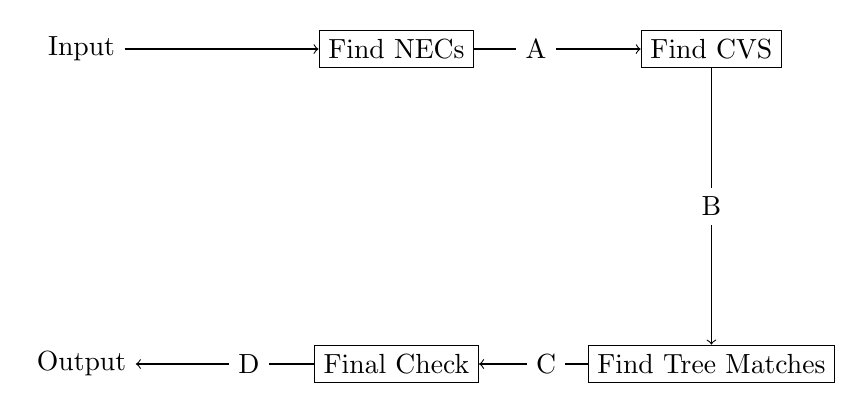
\begin{tikzpicture}[node distance=4cm]
\node[draw=none](6)[]{Input};
\node[rectangle,draw] (1)[right of=6]{Find NECs};
\node[rectangle,draw] (2)[right of=1]{Find CVS};
\node[rectangle,draw] (3)[below of=2]{Find Tree Matches};
\node[rectangle,draw] (4)[left of=3]{Final Check};
\node[draw=none](5)[left of =4]{Output};
\path[->]
	(6) edge node{} (1)
	(1) edge node[minimum width = 1em, fill = white,pos=.25,right] {A} (2)
	(2) edge node[minimum width = 1em, fill = white,pos=.5]{B} (3)
	(3) edge node[minimum width = 1em, fill = white,pos=.2,left]{C} (4)
	(4) edge node[minimum width = 1em, fill = white,pos=.25,left] {D} (5);
\end{tikzpicture}

 \caption{Intermediate Answers}
\end{figure}
	 $A$, $B$, $C$, $D$ are the intermediate answer saved variables. $A$ store the NECs of each vertex in query graph. $B$ store CVS of each query vertex in data graph. $C$ store the possible tree matches. $D$ store the final exact graph maps.
\section{Adding Edge to Query Graph}
 \label{sec:aq}
	\hspace{10mm} Its one of the easiest case because we need to check only the previous cases. The final answer will be a subset of previous answer,ie.,matching will become invalid when the added edge is not present. Only D changes. Multiple queries can be done in parallel  by checking the existence of the added edges in all the previous answers. In parallel, on all previous answers check the presence of added edges.
\section{Deleting Edge from Data Graph}
 \label{sec:dd}
	\hspace{10mm} It is also easy because the final answer is subset of previous answer.Multiple Queries can be processed similiar to the previous case.Only D changes.
\section{Deleting Edge from Query Graph}
 \label{sec:dq}
	\hspace{10mm} This is a difficult case since we need to find the mappings that are going to be added. 
\begin{figure}[h]
 \centering
	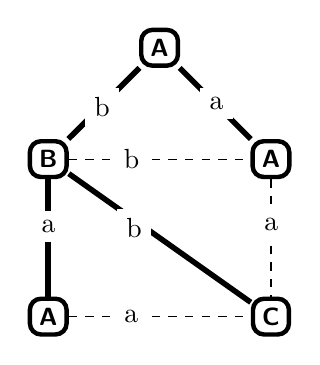
\begin{tikzpicture}[node distance=2cm,node/.style={rounded corners,draw,font=\sffamily\small\bfseries}]
	\node[node,line width=1.6pt] (1) {A};
	\node[node,line width=1.6pt] (2)[below left of=1] {B};
		\node[node,line width=1.6pt] (3)[below right of=1] {A};
		\node[node,line width=1.6pt] (4)[below  of=2] {A};
			\node[node,line width=1.6pt] (5)[below of=3] {C};
	\path
	(1) edge[line width=.7mm] node [minimum width = 1em, fill = white,pos=.25,below left] {b} (2)
		edge[line width=.7mm] node [minimum width = 1em, fill = white,pos=.25,below right]{a} (3)	
	(2) edge[dashed] node [minimum width = 1em, fill = white,pos=.25,right]{b} (3)
		edge[line width=.7mm] node [minimum width = 1em, fill = white,pos=.25,below]{a} (4)
		edge[line width=.7mm] node [minimum width = 1em, fill = white,pos=.25,below right]{b} (5)
	(3) edge[dashed] node [minimum width = 1em, fill = white,pos=.25,below]{a} (5)	
	(4) edge[dashed] node [minimum width = 1em, fill = white,pos=.25,right]{a} (5);	
							
\end{tikzpicture}
 \caption{Tree in Query Grpah}
 \label{fig:tree}
\end{figure}
 The deleting an edge in query graph can be divided as deleting any of the dashed edges(non-tree edges) and deleting one of the bold edges(tree edges) in figure \ref{fig:tree}.
\subsection{Deleting a non-tree edge}	
	\hspace{10mm} The tree inside the query graph remains unchanged. So the tree matches are correct. We need to go through all the tree matching(C) and check for possible additions of maps to final answer. So saving the intermediate answer C helps in finding the solution faster.
\subsection{Deleting a tree edge}	
	\hspace{10mm} Since the tree is changed here the CVS of vertices may change. So rather than calculating all the CVS there is a more efficient way. If a edge u-v in the tree is deleted and u is parent of v in tree. All the nodes in the path from u to root(parent,grand-parent,.. of u) should recalculate the CVS.\\
	 \hspace{10mm} When multiple queries are given the deletion may be from different parts of the tree. But each node should be processed once. 
\begin{algorithm}[H]
\caption{Dynamic tree edge deletion of thread t}
\textbf{Input}: Data Graph $D$,Query Graph $Q$,Delete u-v(u is parent of v).\\
\textbf{Output}: CVS updates.\\
\begin{algorithmic}
 \item \begin{enumerate}
 \item w=v
\item for each parent of w(till root)
 \begin{enumerate}
\item mark w for t
\end{enumerate}
\item for each parent of w(till root)
 \begin{enumerate}
\item if mark at w is t, acquire lock for w
\end{enumerate}
\item for each parent of w(till root)
\begin{enumerate}
\item if mark at w is t and able to acquire locks for all childs of w 
\item Recompute NEC of w
\item if not a previously computed NEC then
\item  \hspace{10mm}C(w)=$FindCandidates$(w,D) update
\item Release all locks
\end{enumerate}
\end{enumerate}
\end{algorithmic}
\label{alg:treeedge}
\end{algorithm}
	\hspace{10mm} The above algorithm marks all the parent nodes from a particular deleted edge. This marking helps to make sure only one thread process one node. The processing will be done such a way that no parent nodes are processed if any  child of the parent is unprocessed. So the processing order will be leaf to root. This will change the values inside A and so as B.\\
\begin{figure}[h!]
 \centering
 \begin{minipage}{.3\textwidth}
	 \centering
	 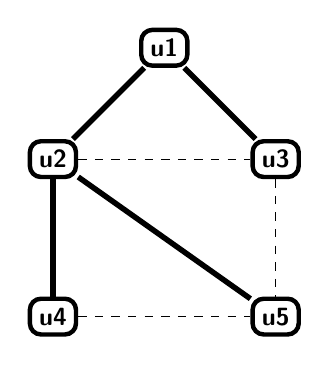
\begin{tikzpicture}[node distance=2cm,node/.style={rounded corners,draw,font=\sffamily\small\bfseries}]
	\node[node,line width=1.6pt] (1) {u1};
	\node[node,line width=1.6pt] (2)[below left of=1] {u2};
		\node[node,line width=1.6pt] (3)[below right of=1] {u3};
		\node[node,line width=1.6pt] (4)[below  of=2] {u4};
			\node[node,line width=1.6pt] (5)[below of=3] {u5};
	\path
	(1) edge[line width=.7mm] node [] {} (2)
		edge[line width=.7mm] node []{} (3)	
	(2) edge[dashed] node []{} (3)
		edge[line width=.7mm] node []{} (4)
		edge[line width=.7mm] node []{} (5)
	(3) edge[dashed] node []{} (5)	
	(4) edge[dashed] node []{} (5);	
							
\end{tikzpicture}
\\\textbf{Step 1}
\end{minipage}
\begin{minipage}{.3\textwidth}
	 \centering
	 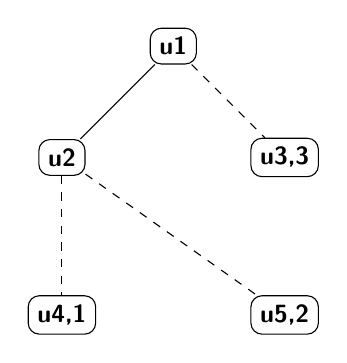
\begin{tikzpicture}[node distance=2cm,node/.style={rounded corners,draw,font=\sffamily\small\bfseries}]
	\node[node] (1) {u1};
	\node[node] (2)[below left of=1] {u2};
		\node[node] (3)[below right of=1] {u3,3};
		\node[node] (4)[below  of=2] {u4,1};
			\node[node] (5)[below of=3] {u5,2};
	\path
	(1) edge[] node [] {} (2)
		edge[dashed] node []{} (3)	
	(2) edge[dashed] node []{} (4)
		edge[dashed] node []{} (5);							
\end{tikzpicture}
\\\textbf{Step 2}
\end{minipage}
\begin{minipage}{.3\textwidth}
	 \centering
	 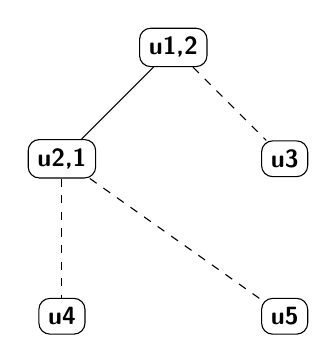
\begin{tikzpicture}[node distance=2cm,node/.style={rounded corners,draw,font=\sffamily\small\bfseries}]
	\node[node] (1) {u1,2};
	\node[node] (2)[below left of=1] {u2,1};
		\node[node] (3)[below right of=1] {u3};
		\node[node] (4)[below  of=2] {u4};
			\node[node] (5)[below of=3] {u5};
	\path
	(1) edge[] node [] {} (2)
		edge[dashed] node []{} (3)	
	(2) edge[dashed] node []{} (4)
		edge[dashed] node []{} (5);							
\end{tikzpicture}
\\\textbf{Step 3}
\end{minipage}\\
\vspace{5mm}
\begin{minipage}{.3\textwidth}
	 \centering
	 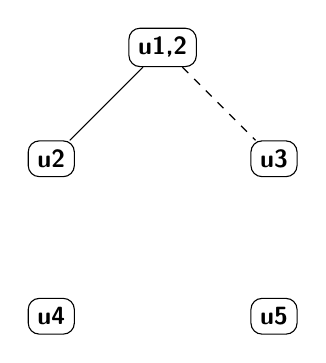
\begin{tikzpicture}[node distance=2cm,node/.style={rounded corners,draw,font=\sffamily\small\bfseries}]
	\node[node] (1) {u1,2};
	\node[node] (2)[below left of=1] {u2};
		\node[node] (3)[below right of=1] {u3};
		\node[node] (4)[below  of=2] {u4};
			\node[node] (5)[below of=3] {u5};
	\path
	(1) edge[] node [] {} (2)
		edge[dashed] node []{} (3);							
\end{tikzpicture}
\\\textbf{Step 4}
\end{minipage}
\begin{minipage}{.3\textwidth}
	 \centering
	 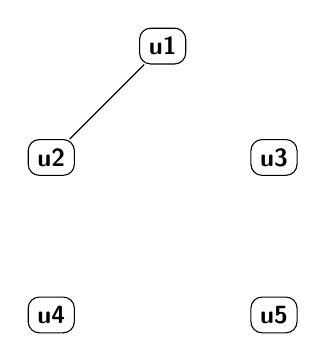
\begin{tikzpicture}[node distance=2cm,node/.style={rounded corners,draw,font=\sffamily\small\bfseries}]
	\node[node] (1) {u1};
	\node[node] (2)[below left of=1] {u2};
		\node[node] (3)[below right of=1] {u3};
		\node[node] (4)[below  of=2] {u4};
			\node[node] (5)[below of=3] {u5};
	\path
	(1) edge[] node [] {} (2);						
\end{tikzpicture}
\\ \textbf{Step 5}
\end{minipage}
 \caption{Deleting Edge in Query Graph}
 \label{fig:deltreeedge}
\end{figure}
\par In Figure \ref{fig:deltreeedge} the tree edge deletion process is shown. The step 1 shows the tree in query graph. Thread 1 deletes u2-u4 edge and thread 2 deletes u2-u5 and thread 3 deletes u1-u3(Step 2 in figure\ref{fig:deltreeedge}). The threads are trying to mark the parents (Step 2 in Algorithm \ref{alg:treeedge}). The marking is not atomic so the thread ids got written in the parents are absolutely random. Here Thread 1 and thread 2 got the parents marked. Since thread 3 doesn't have any parent marked (Step 4(a) in Algorithm\ref{alg:treeedge}), it will return. Now thread 1 will acquire lock on u2 and thread 2 will acquire lock on u1(Step 3 in figure\ref{fig:deltreeedge}). Now thread 2 will go to waiting since it can't attain the lock on u1 's children. So only thread 1 is now processing. It will acquire locks on its children(step 4 in figure\ref{fig:deltreeedge}). Since all of its children are deleted, no locks are required. So thread 1 will recalculate the NEC of u2 and find the candidates in Data graph. After that thread 1 will release the lock and return. Now thread 2 will acquire the locks of all children of u1(step 5 in figure\ref{fig:deltreeedge}). Then it will recalculate the NEC , CVS and finishes.
\section{Adding Edge in Data Graph}
 \label{sec:ad}
	\hspace{10mm} This will also add entries into B. But A will not be changed since no edges in query graph is changed. 
	\begin{algorithm}[H]
\caption{Dynamic data edge addition of thread t}
\textbf{Input}: Data Graph $D$,Query Graph $Q$,Delete u-v(u is parent of v).\\
\textbf{Output}: CVS updates.\\
\begin{algorithmic}
 \item \begin{enumerate}
 \item w=v (for u also)
\item for each child of w(till $|Q|$ length)
\begin{enumerate}
\item if acquire locks for all children of w and w 
\item foreach NEC's as x and w is not in $CVS(x)$
\item \hspace{10mm}$CVS(x)$=$Is_w_candidate$(w,x,D) update
\item Release all locks
\end{enumerate}
\end{enumerate}
\end{algorithmic}
\label{alg:adddataedge}
\end{algorithm}
\hspace{10mm} This algorithm moves to  $|Q|$ length from both u and v in a BFS fashion. At each Data node it is checked whether it can be added to CVS of any of the NECs. When there is an overlap of regions of different thread locks are used to synchronize them. Since the Data graph is huge and  query graph is small and so the possibility of two edge addition happening near( edge length  $< ~|Q|$ ) is small, the number of locks waits will be minimal.
\begin{figure}[h!]
\begin{minipage}{.4\textwidth}
	\centering
	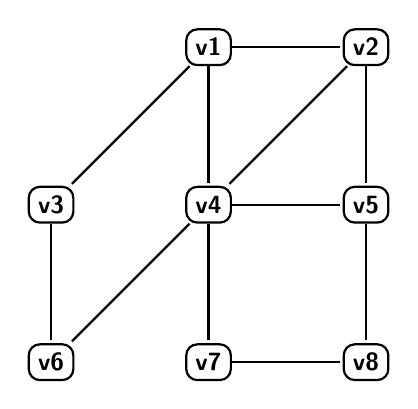
\begin{tikzpicture}[shorten >=1pt,auto,node distance=2cm,
                    thick,main node/.style={rounded corners,draw,font=\sffamily\small\bfseries}]

  \node[main node] (1) {v1};
  \node[main node] (2) [right of=1] {v2}; 
  \node[main node] (4) [below of =1] {v4};
  \node[main node] (3) [left of=4] {v3};
     \node[main node] (5) [below of=2] {v5};
    \node[main node] (6) [below of=3] {v6};
    \node[main node] (7) [below of=4] {v7};
\node[main node] (8) [below of=5] {v8};
  \path[every node/.style={font=\sffamily\small}]
    (1) edge[] node [] {} (2)
        edge[] node[] {} (3)
        edge[] node[] {} (4)
    (2) edge[] node [] {} (4)
        edge node [] {} (5)
    (3) edge[] node [] {} (6)
    (4) edge node [] {} (7)
    	edge[] node [] {} (6) 
    	edge node [] {} (5) 
    (5) edge node [] {} (8)
    (7) edge node [] {} (8);	   
\end{tikzpicture}
\\\textbf{Step 1}
\end{minipage}
\begin{minipage}{.4\textwidth}
	\centering
	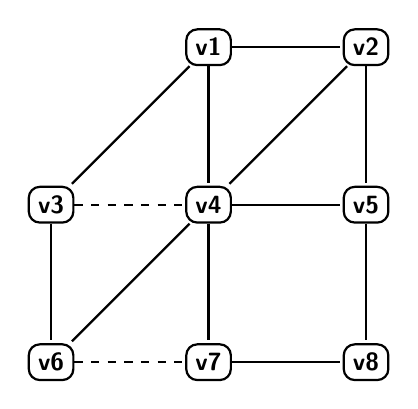
\begin{tikzpicture}[shorten >=1pt,auto,node distance=2cm,
                    thick,main node/.style={rounded corners,draw,font=\sffamily\small\bfseries}]

  \node[main node] (1) {v1};
  \node[main node] (2) [right of=1] {v2}; 
  \node[main node] (4) [below of =1] {v4};
  \node[main node] (3) [left of=4] {v3};
     \node[main node] (5) [below of=2] {v5};
    \node[main node] (6) [below of=3] {v6};
    \node[main node] (7) [below of=4] {v7};
\node[main node] (8) [below of=5] {v8};
  \path[every node/.style={font=\sffamily\small}]
    (1) edge[] node [] {} (2)
        edge[] node[] {} (3)
        edge[] node[] {} (4)
    (2) edge[] node [] {} (4)
        edge node [] {} (5)
    (3) edge[] node [] {} (6)
    	edge[dashed] node []{} (4)
    (4) edge node [] {} (7)
    	edge[] node [] {} (6) 
    	edge node [] {} (5) 
    (5) edge node [] {} (8)
    (6) edge[dashed] node[] {} (7)
    (7) edge node [] {} (8);	   
\end{tikzpicture}
\\\textbf{Step 2}
\end{minipage}\\
\hfill\vspace{5mm} \hfill\\
\begin{minipage}{.4\textwidth}
	\centering
	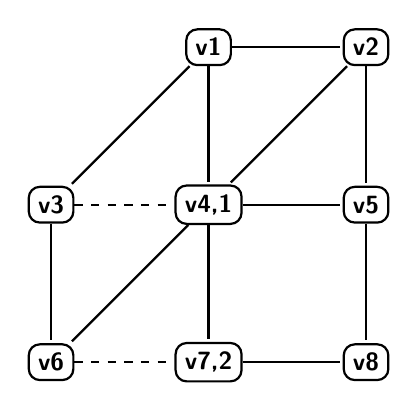
\begin{tikzpicture}[shorten >=1pt,auto,node distance=2cm,
                    thick,main node/.style={rounded corners,draw,font=\sffamily\small\bfseries}]

   \node[main node] (1) {v1};
  \node[main node] (2) [right of=1] {v2}; 
  \node[main node] (4) [below of =1] {v4,1};
  \node[main node] (3) [left of=4] {v3};
     \node[main node] (5) [below of=2] {v5};
    \node[main node] (6) [below of=3] {v6};
    \node[main node] (7) [below of=4] {v7,2};
\node[main node] (8) [below of=5] {v8};
  \path[every node/.style={font=\sffamily\small}]
    (1) edge[] node [] {} (2)
        edge[] node[] {} (3)
        edge[] node[] {} (4)
    (2) edge[] node [] {} (4)
        edge node [] {} (5)
    (3) edge[] node [] {} (6)
    	edge[dashed] node []{} (4)
    (4) edge node [] {} (7)
    	edge[] node [] {} (6) 
    	edge node [] {} (5) 
    (5) edge node [] {} (8)
    (6) edge[dashed] node[] {} (7)
    (7) edge node [] {} (8);	   
\end{tikzpicture}
\\\textbf{Step 3}
\end{minipage}
\begin{minipage}{.4\textwidth}
	\centering
	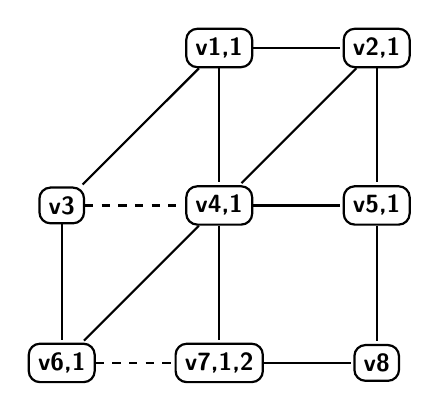
\begin{tikzpicture}[shorten >=1pt,auto,node distance=2cm,
                    thick,main node/.style={rounded corners,draw,font=\sffamily\small\bfseries}]

  \node[main node] (1) {v1,1};
  \node[main node] (2) [right of=1] {v2,1}; 
  \node[main node] (4) [below of =1] {v4,1};
  \node[main node] (3) [left of=4] {v3};
     \node[main node] (5) [below of=2] {v5,1};
    \node[main node] (6) [below of=3] {v6,1};
    \node[main node] (7) [below of=4] {v7,1,2};
\node[main node] (8) [below of=5] {v8};
  \path[every node/.style={font=\sffamily\small}]
    (1) edge[] node [] {} (2)
        edge[] node[] {} (3)
        edge[] node[] {} (4)
    (2) edge[] node [] {} (4)
        edge node [] {} (5)
    (3) edge[] node [] {} (6)
    	edge[dashed] node []{} (4)
    (4) edge node [] {} (7)
    	edge[] node [] {} (6) 
    	edge node [] {} (5) 
    (5) edge node [] {} (8)
    (6) edge[dashed] node[] {} (7)
    (7) edge node [] {} (8);	   
\end{tikzpicture}
\\\textbf{Step 4}
\end{minipage}\\
\hfill \vspace{5mm}\hfill \\
\begin{minipage}{.4\textwidth}
	\centering
	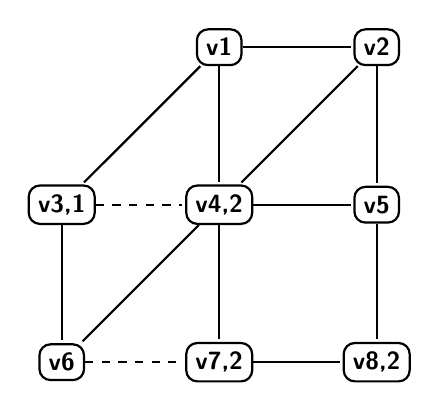
\begin{tikzpicture}[shorten >=1pt,auto,node distance=2cm,
                    thick,main node/.style={rounded corners,draw,font=\sffamily\small\bfseries}]

  \node[main node] (1) {v1};
  \node[main node] (2) [right of=1] {v2}; 
  \node[main node] (4) [below of =1] {v4,2};
  \node[main node] (3) [left of=4] {v3,1};
     \node[main node] (5) [below of=2] {v5};
    \node[main node] (6) [below of=3] {v6};
    \node[main node] (7) [below of=4] {v7,2};
\node[main node] (8) [below of=5] {v8,2};
  \path[every node/.style={font=\sffamily\small}]
    (1) edge[] node [] {} (2)
        edge[] node[] {} (3)
        edge[] node[] {} (4)
    (2) edge[] node [] {} (4)
        edge node [] {} (5)
    (3) edge[] node [] {} (6)
    	edge[dashed] node []{} (4)
    (4) edge node [] {} (7)
    	edge[] node [] {} (6) 
    	edge node [] {} (5) 
    (5) edge node [] {} (8)
    (6) edge[dashed] node[] {} (7)
    (7) edge node [] {} (8);	   
\end{tikzpicture}
\\\textbf{Step 5}
\end{minipage}
\begin{minipage}{.4\textwidth}
	\centering
	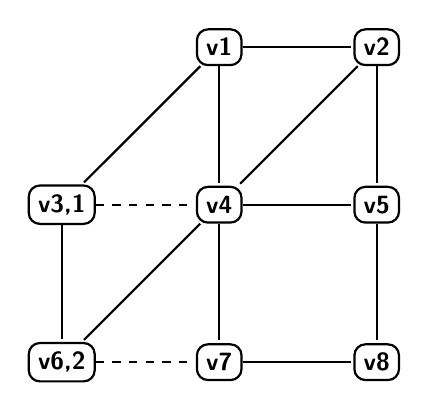
\begin{tikzpicture}[shorten >=1pt,auto,node distance=2cm,
                    thick,main node/.style={rounded corners,draw,font=\sffamily\small\bfseries}]

  \node[main node] (1) {v1};
  \node[main node] (2) [right of=1] {v2}; 
  \node[main node] (4) [below of =1] {v4};
  \node[main node] (3) [left of=4] {v3,1};
     \node[main node] (5) [below of=2] {v5};
    \node[main node] (6) [below of=3] {v6,2};
    \node[main node] (7) [below of=4] {v7};
\node[main node] (8) [below of=5] {v8};
  \path[every node/.style={font=\sffamily\small}]
    (1) edge[] node [] {} (2)
        edge[] node[] {} (3)
        edge[] node[] {} (4)
    (2) edge[] node [] {} (4)
        edge node [] {} (5)
    (3) edge[] node [] {} (6)
    	edge[dashed] node []{} (4)
    (4) edge node [] {} (7)
    	edge[] node [] {} (6) 
    	edge node [] {} (5) 
    (5) edge node [] {} (8)
    (6) edge[dashed] node[] {} (7)
    (7) edge node [] {} (8);	   
\end{tikzpicture}
\\\textbf{Step 6}
\end{minipage}
\caption{Edge Addition Data Graph Processing}
 \label{fig:workingdg}
\end{figure}
\par Step 1 in figure \ref{fig:workingdg} is the data graph. Then 2 edges are added (v6-v7 and  v3-v4). Thread 1 starts processing the v3-v4 edge and Thread 2 starts processing v6-v7 edge(Step 3). Since these edges are so close to each other. There will be lots of waits on locks. The acquire lock on w and children of w in step 2(a) of Algorithm \ref{alg:adddataedge} becomes very complex. The lower id threads are given priority when trying to acquire locks. So the thread 1 acquires lock of v4 and its neighbors(Step 4). Thread 2 goes to waiting. The locking system can be implemented using an array with atomic operations. Minimum value write operation will help to give lower threads more priority than higher ones. Now thread 1 will recalculate the CVS changes for all NEC for which v4 is not a part of. Now thread 1 will move to other end of the edge (v3). Now thread 2 can acquire locks on v7 and its neighbors(Step 5). Thread 2 will now update the CVS. There is another possibility that thread 1 will ask for lock on v4 because it is a neighbor of v3. Then thread 2 can again go to waiting. These lock waitings are happening because of closeness of both added edges. So now thread 2 will move to v6(Step 6). Then the process continues. Thread 1 will go through v4, v3, v1, v2, v5, v7 and v6. Since it should go through all the nodes at a 2 hopes(length of query tree). Similiarly thread 2 will go through v7, v6, v4,v8 and v3.
\subsection{Parallel Execution}
\hspace{10mm} All the four quires can be processed in parallel since they are operating on different data.Section \ref{sec:aq} and \ref{sec:dd} are processing on D while Section \ref{sec:dq} and \ref{sec:ad} are processing on A and B. So it is safe to run in parallel. Parallel adding to A and B doesn't make the answer inconsistent. It will add a vertex into the CVS which  will be removed when exact matching is performed in the end.
\subsection{Inferences}
	\hspace{10mm} So a $Find Tree$ match algorithm should be done at each stage of the output to get the new results . But this stage is the costliest of all the four steps. Even if one vertex is added to any two CVS, we need to recompute most of the permutations again. So there is no computational advantage by dynamic processing. Running a sub-graph isomorphism solution after applying all edge updates becomes equally fast as the dynamic version. 
